\documentclass{beamer}
\usepackage{amssymb}
\usepackage{comment}
\usepackage{multicol}
\usepackage{minted}
\usepackage{makecell}
\usepackage{amsfonts}
\usepackage{booktabs}
\usepackage{siunitx}
\usepackage{graphicx}
\usepackage{amsmath}
\usepackage{xcolor, colortbl}
\usepackage{eso-pic}
\beamertemplatenavigationsymbolsempty


\definecolor{Gray}{gray}{0.9}

%\newcommand{\myitem}{\item[$\blacktriangleright$]}
\newcommand{\myitem}{\item[\triangleright]}

\usetheme[progressbar = frametitle]{metropolis}
\setbeamertemplate{frame numbering}[fraction]
\useoutertheme{metropolis}
\useinnertheme{metropolis}
\usefonttheme{metropolis}
\usecolortheme{dove}
%\usecolortheme{spruce}
\setbeamercolor{background canvas}{bg = white}
%\usepackage[utf8]{inputenc}

\title{Optimal lookback period for momentum on country ETFs}
\author{Ana Jazbinsek, Thomas Meier}
%\institute{University of Zurich}
\date{December 11, 2024}
\titlegraphic{%
  \begin{picture}(0,0)
    \put(142,-175){\makebox(0,0)[rt]{
\includegraphics[width=5cm]{figures/uzh_logo_text.png}}}
  \end{picture}}

\setbeamercovered{transparent = 15}

\begin{document}
\metroset{block=fill}



\begin{comment}
Provisional ToC:

1. Data Cleaning (3min) Robert
1.1 Why we concatenated the data like this.
1.2 Dealing with NaN (Threshold & Knn-Imputer)
1.3 Dealing with outliers
1.4 Handling Class imbalance

2. Feature Selection & Feature Engineering (2min) Thomas
2.1 Feature Engineering With SGM
2.2 Feature Selection with Gradient Boosting -> Feature Importance (Sector very important) -> deshalb kein SMOTE da drop nicht möglich

3. Model Fits & Results (3min) Jan
3.1 Correlation Matrix
3.2 Results, Scaling , Oversampling, Scorer, 
--> Table paste

4. Discussing Results in light of finance theory (2min) Simon
4.1 Market unbeatable (differentiate)
4.2 Fama EMH
4.2 OVB

\end{comment}





\begin{frame}
    \titlepage
\end{frame}
\newcommand\AtPagemyUpperLeft[1]{\AtPageLowerLeft{%
\put(\LenToUnit{0.82\paperwidth},\LenToUnit{0.91\paperheight}){#1}}}
\AddToShipoutPictureFG{
  \AtPagemyUpperLeft{{
\includegraphics[width=2cm,keepaspectratio]{figures/uzh_logo_text.png}}}
}%

\begin{frame}[t]{Introduction}
    \begin{itemize}
        \myitem Cross-sectional momentum strategies: Rank assets by past performance - long top performers, short underperformers.
        \myitem Key Strategy Parameter: Lookback Period
        \begin{itemize}
            \item Determines the timeframe for assessing past performance.
            \item Impacts effectiveness by identifying genuine trends versus anomalies.
        \end{itemize}
    \end{itemize}
    \textbf{Project Focus:} Analyzes lookback periods up to 24 months for country equity momentum strategies.  
    Implements a long-only strategy targeting top three performers.

    \textbf{Customizable parameters:} lookback periods, number of positions, transaction costs, investment universe, period of observation
\end{frame}

\begin{frame}[t]{Momentum Investing Overview}
    \begin{itemize}
        \myitem Jegadeesh and Titman (1993) found that stocks with strong past returns (3-12 months) tend to keep outperforming, challenging the efficient market hypothesis (Fama, 1970).
        \myitem This effect has been observed across various asset classes (Asness et al., 2013; Baltas \& Kosowski, 2013).
        \myitem Explanations for Momentum:
        \begin{itemize}
            \item Behavioral: Investor biases, like delayed reactions, lead to price continuation (Barberis et al., 1998; Grinblatt \& Han, 2005).
            \item Risk-Based: Momentum profits may compensate for systematic risks not captured by traditional models (Bikhchandani et al., 1992).
        \end{itemize}
    \end{itemize}
\end{frame}


\begin{frame}[t]{Data}
We used the \textbf{Yahoo finance API} to pull daily price data on 17 country ETFs: USA, China, Japan, India, Brazil, Canada, Mexico, South Korea, Germany, UK, Australia, Switzerland, Hong Kong, Singapore, Taiwan, Italy, Spain. 

We transformed this into a monthly return series that we use for the strategy.

We also pull the data for the risk free rate from Yahoo finance, taking the 3-month US treasury yield as risk free.
\end{frame}

\begin{frame}[t]{Momentum Strategy Overview}
    \begin{itemize}
        \item Momentum investing: Strategy based on past trends predicting future returns.
        \item Momentum defined as the return difference over a specified lookback period $h$.
        \item Equation for momentum calculation:
        \begin{equation}
            MOM_{t,i} = r_{t-1,i} - r_{t-h,i}
        \end{equation}
    \end{itemize}
\end{frame}

\begin{frame}[t]{Weighting Strategy}
    \begin{itemize}
        \item Long-only strategy: Assign equal weight $\frac{1}{k}$ to the top $k$ ETFs based on momentum.
        \item Long-short strategy: Allocate weights for top $k$ long ETFs and bottom $k$ short ETFs.
        \item Weight calculation equations:
        \begin{align}
            w_{t,i} &= \begin{cases} 
            \frac{1}{k} & \text{if top } k \text{ at time } t \\
            0           & \text{otherwise}
            \end{cases} \\
            w_{t,i} &= \begin{cases} 
            \frac{1}{k}  & \text{if top } k \text{ (long) at time } t \\
            -\frac{1}{k} & \text{if bottom } k \text{ (short) at time } t \\
            0            & \text{otherwise}
            \end{cases}
        \end{align}
    \end{itemize}
\end{frame}


\begin{frame}[t]{Transaction Costs and Adjustments}
    \begin{itemize}
        \item Account for transaction costs: Proportional cost $c$ per unit.
        \item Adjust for returns between rebalancing:
        \begin{equation}
            \hat{w}_{t,i} = w_{t-\epsilon,i} \frac{1 + r_{t,i}}{1 + r_{t,PF}}
        \end{equation}
        \item Calculate turnover $z_t$:
        \begin{equation}
            z_{t} = \sum_{j=1}^{K}\lvert w_{t,i} - \hat{w}_{t,i} \rvert
        \end{equation}
        \item Total turnover cost: $z_t \cdot c$ deducted from monthly return.
    \end{itemize}
\end{frame}

\begin{frame}[t]{Benchmark}
    \begin{itemize}
        \item Equally weighted over the whole investment universe - passive investment.
        \item Monthly rebalancing to stay equally weighted. This incurs transaction costs.
    \end{itemize}
\end{frame}


\begin{frame}[t]{Empirical results}
    \begin{figure}[t!]\centering
    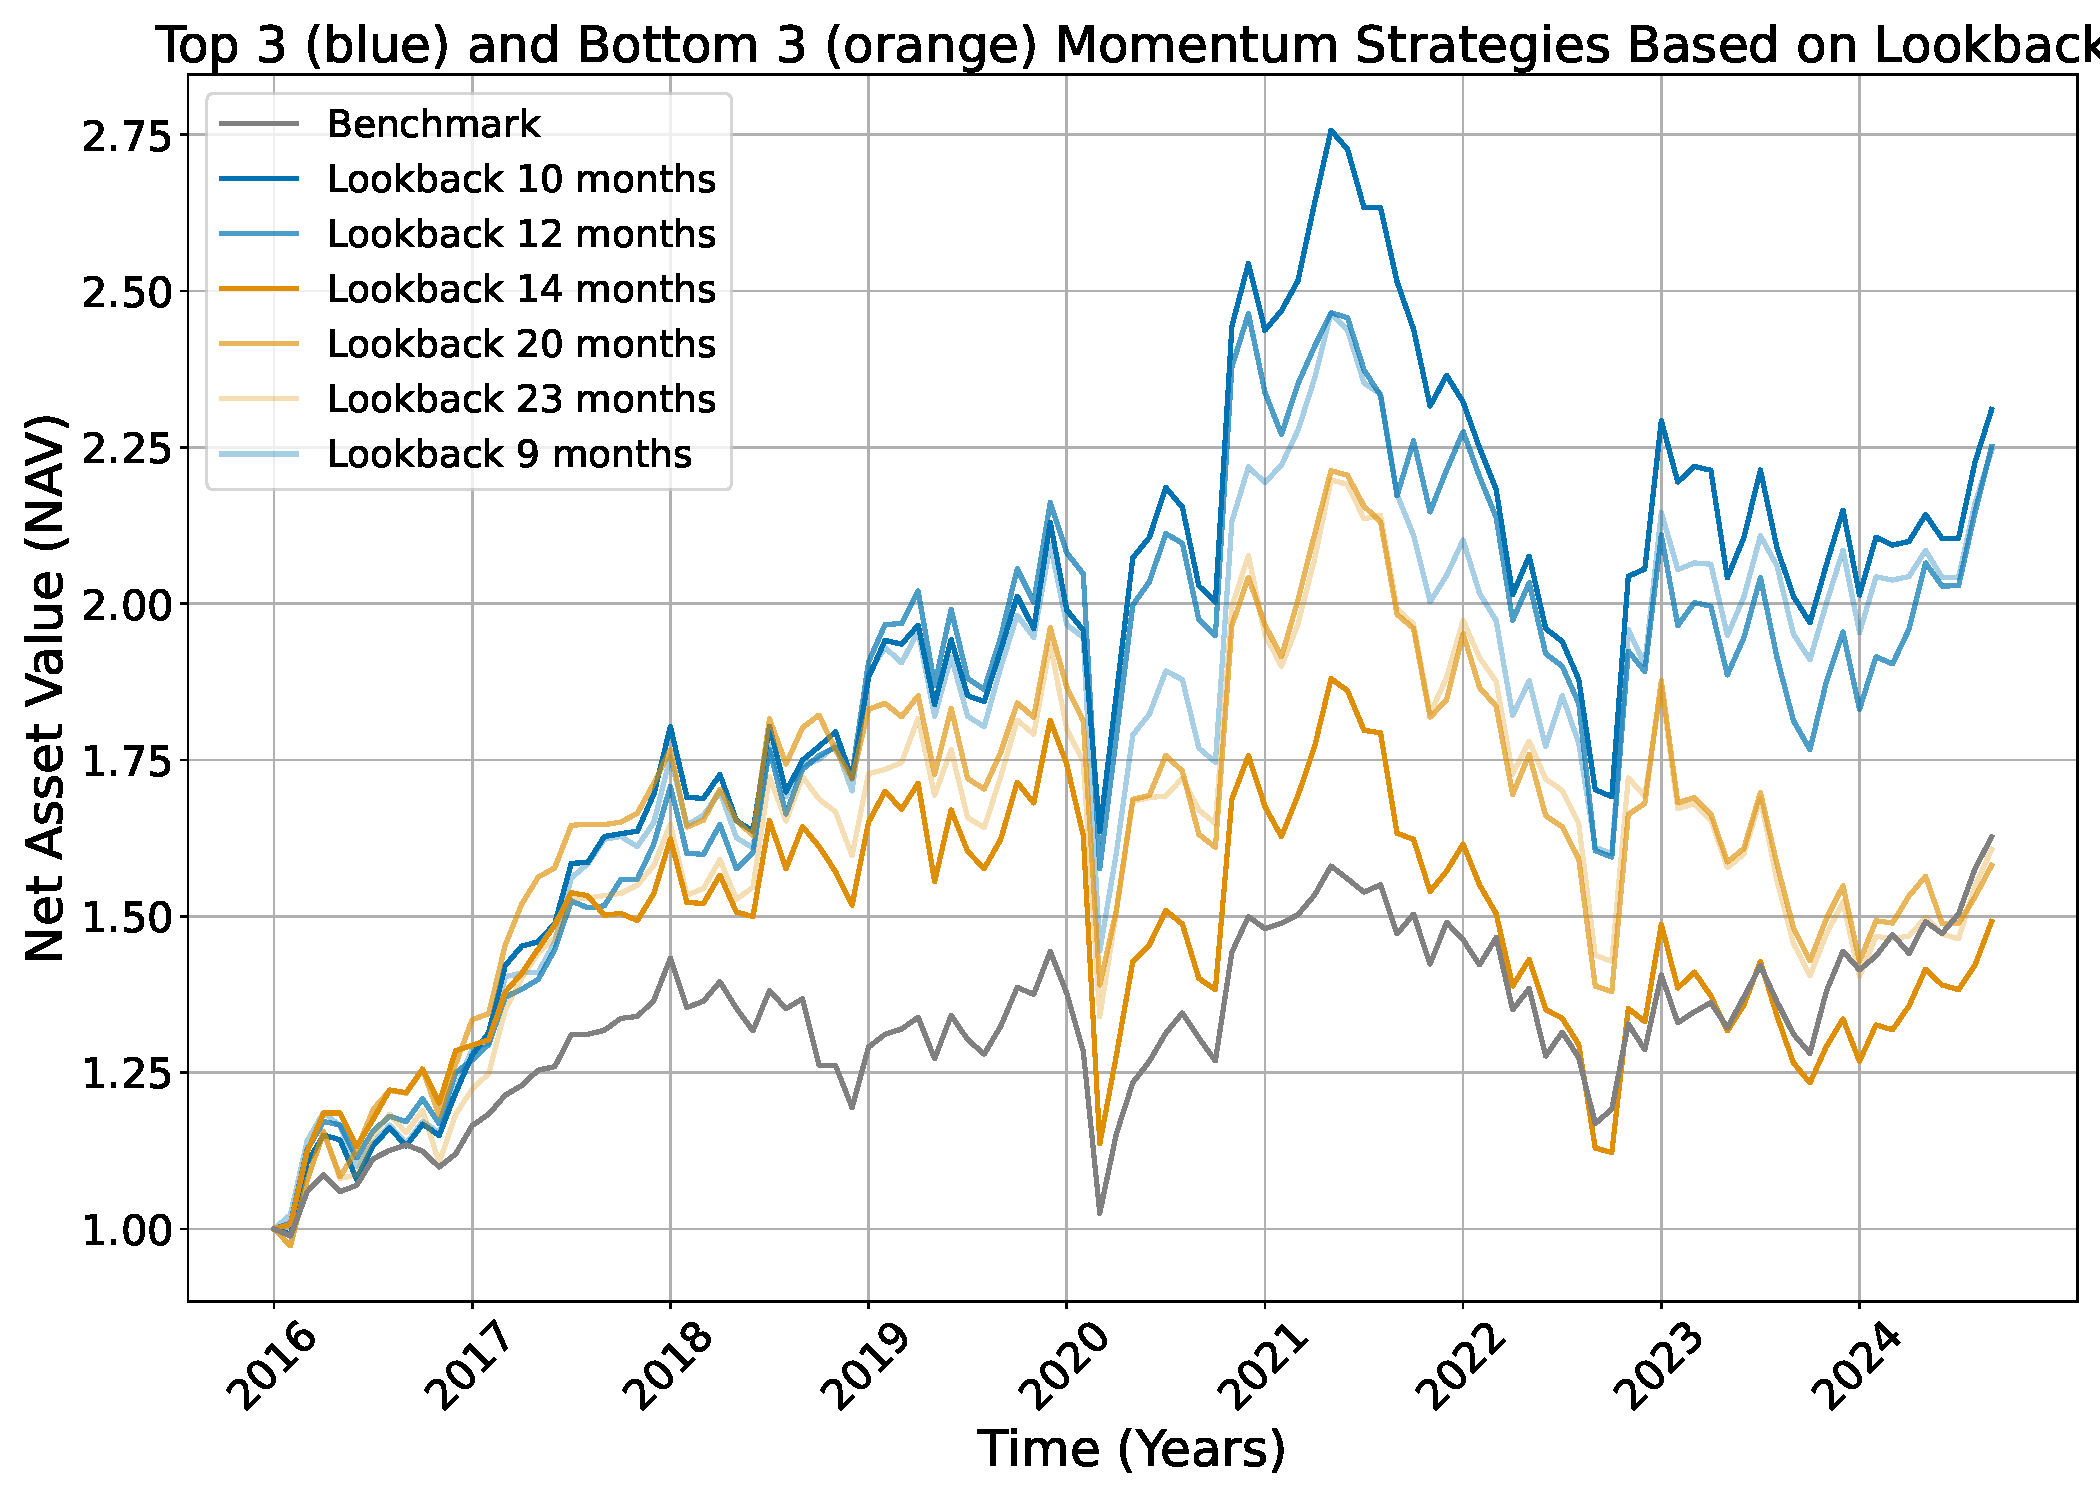
\includegraphics[width=10cm]{figures/fig_bm.pdf}
    \centering
   %% \caption[caption]{Sustainable Growth Model according to Higgins}
    \label{fig_bm}
    \end{figure}
    
\end{frame}

\begin{frame}[t]{Empirical results}
    \begin{figure}[t!]\centering
    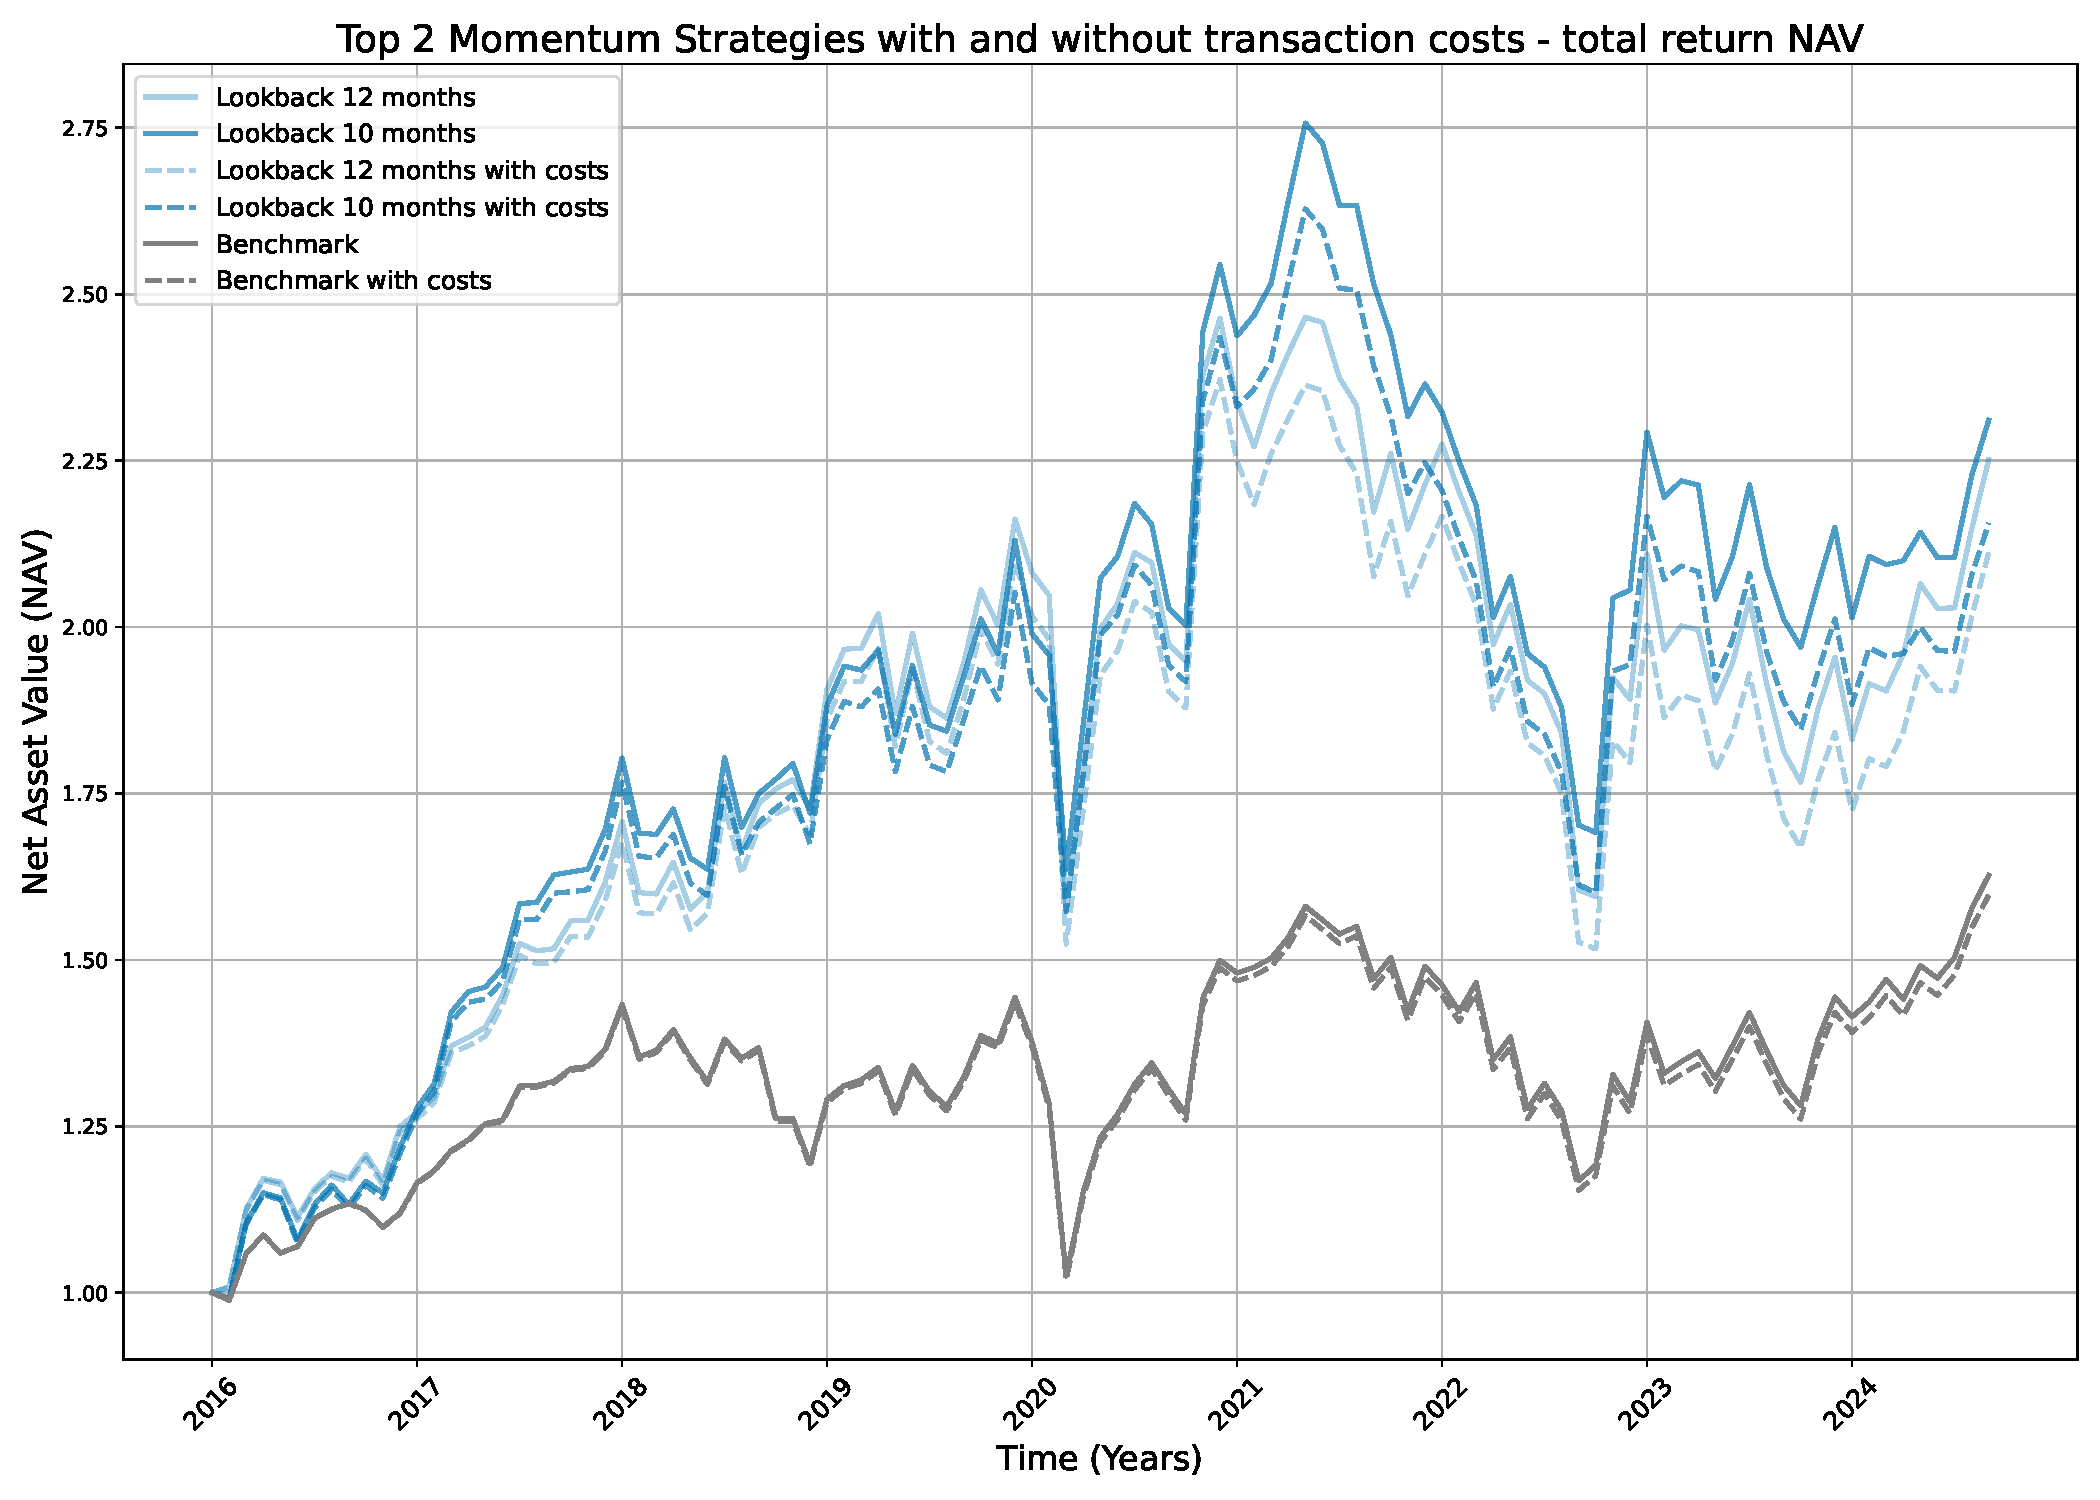
\includegraphics[width=10cm]{figures/fig_costs.pdf}
    \centering
   %% \caption[caption]{Sustainable Growth Model according to Higgins}
    \label{fig_costs}
    \end{figure}
    
\end{frame}

\begin{frame}[t]{Conclusion}
    \begin{itemize}
        \myitem Shorter lookback periods (up to 12 months) generally outperform longer periods, consistent with literature on diminishing predictive power of extended lookbacks.
        \myitem Best momentum strategies outperform passive benchmarks, even after accounting for transaction costs. Momentum strategies incur higher turnover and transaction costs than benchmarks but still deliver significant risk-adjusted returns.
    \end{itemize}

    This study confirms momentum as a reliable and effective strategy for country ETFs.
\end{frame}

\begin{frame}[t]{References}
    \begin{figure}[t!]\centering
    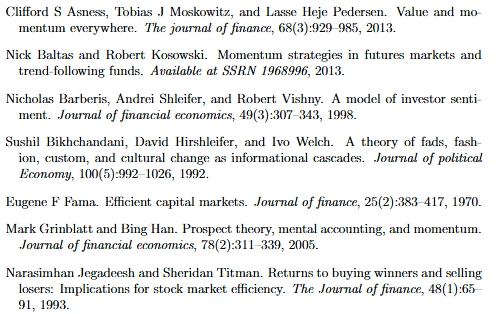
\includegraphics[width=10cm]{figures/ref1.PNG}
    \centering
   %% \caption[caption]{Sustainable Growth Model according to Higgins}
    \label{ref1}
    \end{figure}
    
\end{frame}

\begin{frame}[t]{References}
    \begin{figure}[t!]\centering
    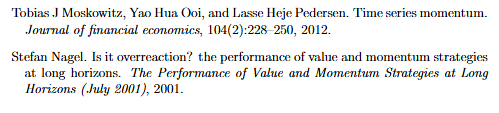
\includegraphics[width=10cm]{figures/ref2.PNG}
    \centering
   %% \caption[caption]{Sustainable Growth Model according to Higgins}
    \label{ref2}
    \end{figure}
    
\end{frame}

\end{document}
